\documentclass[journal,a4paper]{IEEEtran}

% to typeset URLs, URIs, and DOIs
\usepackage[english]{babel}
\usepackage{url}
\usepackage{multicol}
\usepackage{multirow}
\usepackage{url,hyperref,graphicx,float,times}
\usepackage{textcomp}
\usepackage{cite}
\usepackage[caption=false,font=footnotesize]{subfig}
\usepackage{amsmath}
\graphicspath{ {./images/} }


\begin{document}
%
\title{Decentralized Data Marketplace to Enable Trusted Machine Economy}
%
\author{
%%% Fill in name here
\IEEEauthorblockN{Ching-Chun (Jim) Huang\IEEEauthorrefmark{1}, Ching-Hua Lin\IEEEauthorrefmark{2}, Zan-Jun Wang\IEEEauthorrefmark{3}}\\

%%% Fill in school here
\IEEEauthorblockA{\IEEEauthorrefmark{1}\IEEEauthorrefmark{2}Department of Computer Science and Information Engineering National Cheng Kung University} \\
\IEEEauthorblockA{\IEEEauthorrefmark{3}Department of Computer Science and Information Engineering National Taiwan University} \\

%%% Fill in address here
\IEEEauthorblockA{\IEEEauthorrefmark{1}\IEEEauthorrefmark{2}No.1, University Road, \IEEEauthorrefmark{3}No.1, Sec. 4, Roosevelt Road} \\

%%% Fill in city and country here
\IEEEauthorblockA{\IEEEauthorrefmark{1}\IEEEauthorrefmark{2}Tainan City, Taiwan (R.O.C.), \IEEEauthorrefmark{3}Taipei City, Taiwan (R.O.C.)} \\

%%% Fill in email here
\IEEEauthorblockA{\IEEEauthorrefmark{1}jserv@ccns.ncku.edu.tw, \IEEEauthorrefmark{2}jkrvivian@gmail.com, \IEEEauthorrefmark{3}twzjwang@gmail.com}
}


%


\maketitle              
% 50-80 words
\begin{abstract}
abstract here
\end{abstract}

% 3 - 4 keywords
\begin{IEEEkeywords}
streaming data, crowd sensing, data marketplace, decentralization
\end{IEEEkeywords}

\section{Introduction}

\section{Related Work}
The increasing IoT devices brings a huge amount of data, the economic value becomes essential for parties intended to sell, buy and find data. The need for IoT data marketplace arises due to this. Recent years, several researchers has started to explore based on this concept. There are some critical issues need to be resolved in the design of data marketplace platform, in this paper, we focus on two issues, data integrity and the trading behavior.

To ensure data integrity for IoT applications is always a challenge because of the unstandardize data format and dynamic nature. Moreover, the Third Party Auditors (TPAs)-based frameworks is far from being satisfactory. Therefore a decentralized data integrity validation has been proposed recent years, and blockchain is considered a solution. 

Data Integrity as a Service (DIaas) is a blockchain based framework for data integrity proposed by Bin Liu\cite{DIaas}. DIaas is a Cloud Server Service (CSS) for IoT dynamic data that allows both data owner and data consumer to validate data integrity by comparing hashes on smart contract  and on Cloud Server. Besides, smart contract can also realize the purchase agreement, including authorizing data consumer for specific data set and even the penalty for data provider if they fail to provide the data integrity. However, the performance analysis shows that IoT devices still have low efficiency interacting with Etheruem, this may fall to the Proof-of-Work (PoW) process is time-consuming for an IoT device and the blockchain consensus can not be reached within a short time, while Ethereum is expected to enable consensus within 12-second but the time is still longer when the authors wrote the paper. 

By solving the inefficiencies of the Blockchain, \textbf{IOTA}\cite{IOTAwhitepaper} is a cryptocurrency for the IoT industry or Web 3.0 based on the revolutionary distributed ledger technology, the \textbf{Tangle}. It is a secure, scalable and feeless transaction settlement layer which enables micropayments transaction. On top of that, \textbf{Masked Authenticated Messaging(MAM)}\cite{MAM}, a second layer data communication protocol which adds functionality to emit and access an encrypted data stream over the Tangle where privacy and integrity meet is introduced to public. On the basis of the Tangle and MAM, IOTA foundation proposed a fully decentralized Data MarketPlace which is suitable for IoT streaming data that not only allow data owners and consumers to trade on Tangle but also protect privacy and assure data integrity from source with MAM. But only the data buyout doesn't meet the need of the real world, such as data subscription and a specific time period of data maybe needed for different uses. Moreover, even though IOTA needs less computing power than other blockchain system, doing PoW and unstable network environment are still the bottleneck for low-level devices, it may take 2 or more minutes to issue a transaction to Tangle under MAM protocol.

A different framework design proposed by Pooja Gupta, Salil S.Kanhere and Raja Jurdak\cite{3tierDataMarket} could solve the efficiency problem as mentioned. The infrastructure is a 3-tier decentralized data marketplace architectural design with smart contract which consists of provider, consumer and broker. Where broker is a highly resourced and trustless device that will facilitate the trading of data between the consumer and providers. However, there are some potential threats need to be resolved, such as payment fairness, authentication of the participants, faithful delivery of data and probable malicious behaviour of data marketplace participants.  

Our proposed data marketplace framework is a 3-tier decentralized and trustless architecture that put data stream and trading process on distrubted ledgers. In our infrastructure, the identity of each participants could be easily verified with a self-soverign identity system, also we design the refunding mechanism to protect the payment fairness. Moreover, with MAM as our data storage on IOTA, data could be delivered securely and faithfully without any third-parties.


\section{System Architecture}
\subsection{Participants}
There are four major roles in the decentralized data marketplace.

\subsubsection{Registrar}
Registrar is responsible for creating a Registration Contract, which maintains a lookup table of participants, and adding new data providers, consumers and brokers to the decentralized data marketplace.

\subsubsection{Data Provider}
Data providers, who generate and preserve IoT data, are willing to sell sensing data to consumers. They decide the subscription period, subscription price, data type, sampling frequency. Afterward, they can launch the product on the decentralized data marketplace. Next, they collect raw data with their sensors and send to the broker who assists in uploading data to the network. An MAM channel\cite{MAM} is used to store encrypted data stream.

\subsubsection{Consumer}
Consumers aspire to obtain IoT data to promote the value of their service. However, it is a big challenge for most consumers to collect the desired data by themselves. So they look forward to purchasing the IoT data from data providers.

\subsubsection{Broker}
Brokers represent data providers and consumers to do computing tasks in the DLT (Distributed Ledger Technology) since brokers are expected to have high computing power. Once a data provider wants to launch a new product, the data provider requests a broker to create a new MAM channel, a new Product Contract, which specifies details about products, and upload this product to a decentralized storage system\cite{IPFS}. Also the broker certifies the session key which is used for symmetric encryption for streaming data encryption and decryption. Then the broker provides the matching service for data provider’s products and consumer’s queries. After that, the broker is requested to deal with the trading process and upload the provider’s data streams to the MAM channel.

\subsection{Component}
\subsubsection{IOTA}
IOTA\cite{IOTAwhitepaper} is a cryptocurrency which the ledger does not consist of transactions grouped into blocks and stored in sequential chains, but a directed acyclic graph(DAG) of individual transactions, \textbf{Tangle}. To issue a transaction in the network, one needs to perform a small amount of Proof-of-Work (PoW) that verifies two previous transactions. Since every actor in Tangle has the same role, there is no need to offer transaction fees. Therefore, it is possible to make \textbf{micropayments} which the importance will increase in the rapidly developing IoT industry, and \textbf{zero-transactions} that one could store information securely within Tangle transactions. Moreover, this structure also enables high scalability of transactions that could resolve the drawbacks of blockchain and the concern of rapid growth of IoT devices.

\subsubsection{Ethereum Smart Contract}
Smart contract\cite{smartContract} is a protocol for formulating agreement on blockchain that provides verification and execution of the contract. The code in the smart contract could interact with other contracts, make decisions, store data and transfer cryptocurrency. All conditions and states established in the contract are transparent and with enforcement. The appearance of smart contracts makes trading more flexible, and achieves more complex trading patterns in reality.

\subsubsection{IPFS}
Inter-Planetary File system(IPFS)\cite{IPFS} is a peer-to-peer network for storing and accessing files, websites, applications, and data in a distributed file system which is not maintained with certain nodes or entities but all IPFS users. In our proposed architecture, brokers are responsible to upload the metadata of products, including title, data provider information and data preview to IPFS in order to provide users with search capabilities to meet the consumers' need.

\subsubsection{Masked Authenticated Messaging}
MAM\cite{MAM} is one of the best features of IOTA, it is a second layer data communication protocol enables to emit and access an encrypted data stream over Tangle network. The consensus algorithm of IOTA ensures data integrity. These properties allow MAM to meet the requirements of both data integrity and privacy.

IOTA only allows one message per transaction and couldn't publish continuous related messages because it is easy for an attacker to issue spam transactions if the same address is used. However, MAM publishes each message to a different addresses, and each can be derived from the previous one, this mechanism protects the channel from spamming and allows us to have access to all information with channel root only. Furthermore, MAM can be used in 3 ways to control visibility and access which are public, restricted and private. In our system, restricted MAM channel is used to achieve data authoriazation between providers and consumers.

\subsubsection{TangleID}
TangleID\cite{TangleID} is a self-soverign identity system based on IOTA, the goal is to establish a solution that do not require any third-party authority to verify an identity and its digital footprint. In TangleID, the digital footprint is converted into digital assets with the principle of Decentralized Identifiers (DIDs)\cite{DID} defined by W3C, and by putting DID documents on MAM makes TangleID a GDPR-Complianced system. Each identity has a public/private key pair recorded on MAM, it is used in digital signature for identity authentication. With every participant in data marketplace registers on TangleID, one can easily verify data provider's identity and data integrity with the public key on the DID document, and that we can ensure the reliability of data sources.


\subsubsection{Blind Signature}
Blind signature\cite{blindSig} is a form of digital signature where the message is blinded before it is signed, and the resulting blind signature can be verified publicly against the original. To perform such a signature, the message is first "blinded" by a random "blinding factor", then passed to a signer to sign. The resulting message, along with the blinding factor, can be later verified with the signer's public key. In our system design, brokers would perform blind signature during the process of adding new products for data providers, in order to upload the secret key of MAM channel to smart contract without knowing it. Furthermore, only one blind-signatured secret key is valid for trading and it is not allowed to be updated. By putting the secret key on smart contract prevents malicious providers trades invalid secret keys to consumers privately. 

\section{Trading Model}
In the following, we describe the data trading process in detail. To participate a data marketplace, data providers and consumers have to register first. Then data provider can launch its product on the marketplace. Once a product is launched, it is searchable and could be traded afterward. The whole trading and refunding process is defined in smart contracts which are easily traceable and irreversible.

\subsection{Participants Registration}
At the beginning, the registrar creates a Registration Contract (Figure \ref{fig:registration_contract}), which maintains all participants' information, including their DID (Decentralized Identifiers) Documents and public keys. Then some trustworthy brokers who pass procedures for conformity assessment are added to the decentralized data marketplace. Anyone who would like to sell or purchase data may register to become the data providers or consumers. The registrar has the authority to agree with applications. After that, their identities are available in the Registration Contract and launching and trading processes can be started.

\begin{figure}[h]
	\centering
	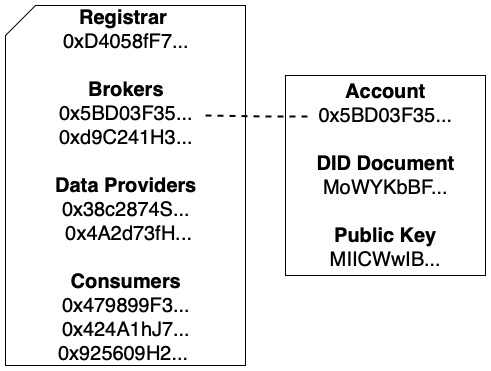
\includegraphics[width=0.4\textwidth]{registration_contract}
	\caption{Registration Contract.}
	\label{fig:registration_contract}
\end{figure}

\subsection{Launching and Searching Products}
To sell the sensing data, a data provider has to launch a new product on the data marketplace in advance. The data provider determines a trusted broker and asks the broker to create a new MAM channel and Product Contract (Figure \ref{fig:product_contract}).

\begin{figure}[h]
\centering
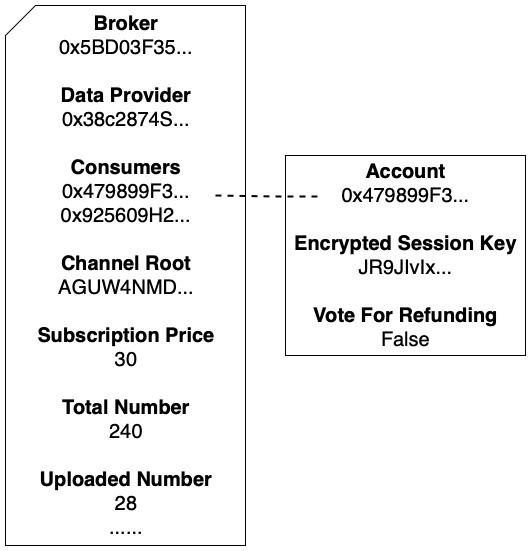
\includegraphics[width=0.4\textwidth]{product_contract}
\caption{Product Contract.}
\label{fig:product_contract}
\end{figure}

Brokers certify session keys as well. Only one session key can be signed in each product, so data providers can't fake a session key to deceive consumers. However, it is a risk revealing session keys to brokers since contents may be copied by brokers, which causes data providers' loss. Therefore, Blind signature is used to prevent the situation. Figure \ref{fig:key_certification} shows the certification process. When a data provider asks a broker to ceritfy new session key $k$, the data provider uses the broker's public key, which is available in the Registration Contract after the broker's registration, as a blinding factor, and the session key is blinded. Then the data provider sends the blinded session key $Blind(k)$ to the broker. The broker signs the message and returns the signature $Sign(Blind(k))$ to data provider. The data provider removes the blinding factor and obtains the broker's signature of the session key, $Sign(k)$, which is verifiable by consumers.

\begin{figure}[h]
	\centering
	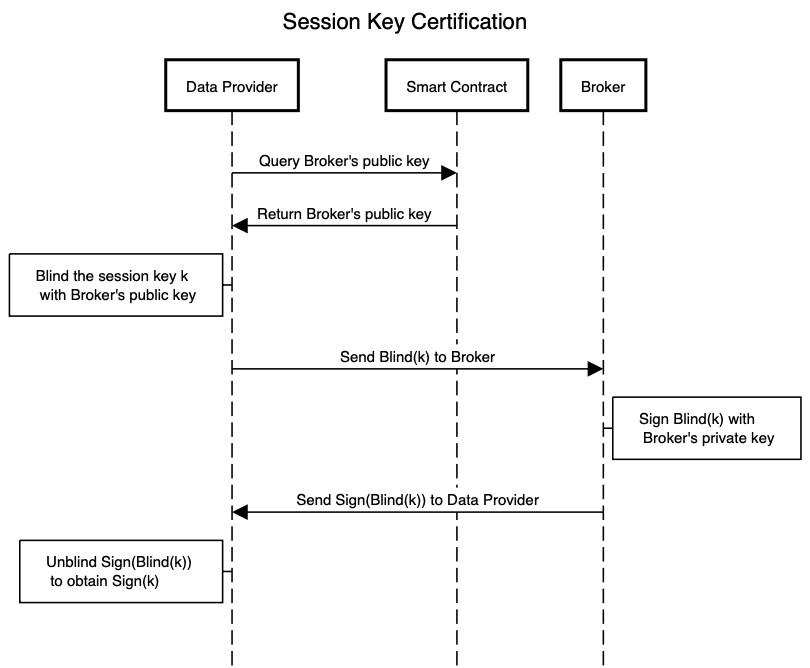
\includegraphics[width=0.5\textwidth]{key_certification}
	\caption{Session key certification process with blind signature.}
	\label{fig:key_certification}
\end{figure}

The contract address and product description will be stored in a file which is uploaded to IPFS. Consumers can search the desired product by keywords or tags. The consumer then evaluates the product and start trading with the data provider if the consumer is interested in subscribing the data.

\subsection{Trading}
Once a consumer who want to subscribe the sensor data pays a subscription fee to the Product Contract, it is added to the consumer list automatically by the smart contract. To decrypt the streaming data on the MAM channel, session key $k$ should be exchanged between data provider and consumers as shown in Figure \ref{fig:key_exchange}. The data provider requests the subscription list maintained by the Product Contract and obtains accounts of each consumer. After that, the data provider can also get public keys of each consumer from the Registration Contract with their accounts. For each consumer, the data provider encrypts the session key and broker's signature with the consumer's public key and sends the ciphertext $Encrypt(k + Sign(k))$ to the Product Contract. Consumers listen to the smart contract event which is triggered when the ciphertext is updated, and decrypt the ciphertext to get the session key $k$ and signature $Sign(k)$. Consumers can obtain the broker's public key on the Registration Contract as well, so they can verify that the signature is valid and the session key is the only one that is certified by the broker. Afterward, encrypted sensing data is uploaded to the MAM channel, and consumers can download and decrypt them with the session key.

\begin{figure}[h]
	\centering
	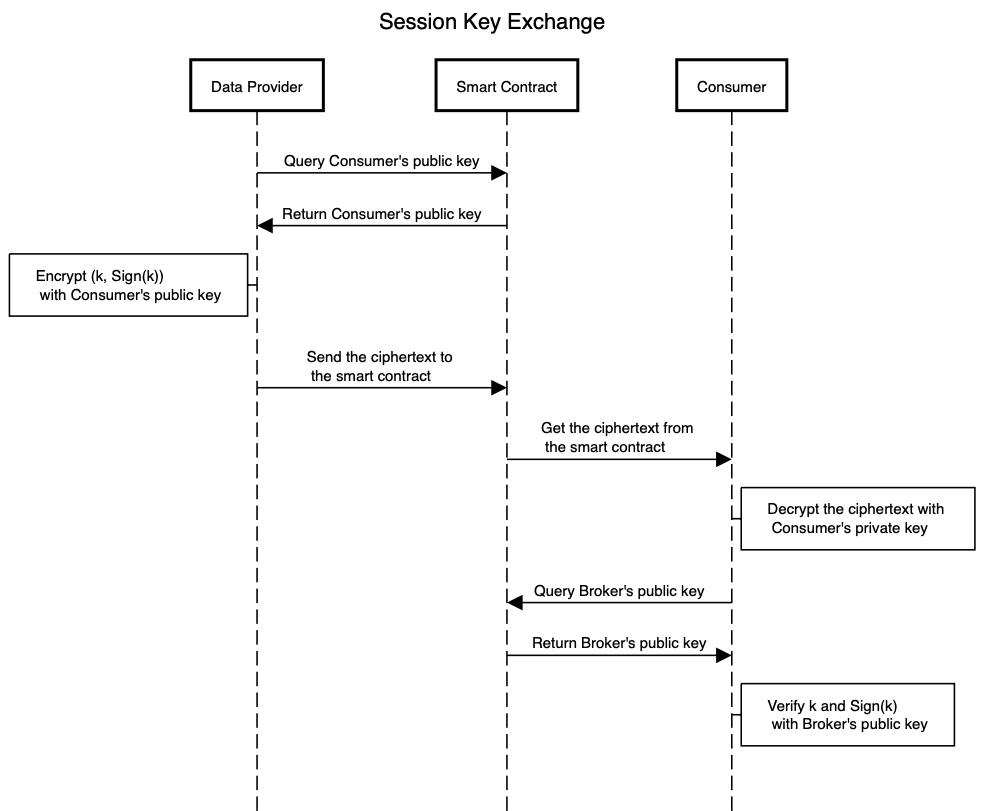
\includegraphics[width=0.5\textwidth]{key_exchange}
	\caption{Session key exchange process between the data provider and consumer.}
	\label{fig:key_exchange}
\end{figure}

\subsection{Refunding}
It is probable that the sensor is malfunctioning after the consumers pay the subscription fee. To protect consumers' right, the subscription fee are not transfered to the data provider until all data is generated and uploaded to the MAM channel. If the expected data is not available, consumers can ask for refunds. We assume that less than half of consumers in the Product Contract are irrational and malicious. Each consumer can vote for refunding at any time. If the ratio of consent votes of refunding is higher than the $threshold$ at $k$th piece of data, the subscription fee is proportionally transfered to the data provider, broker and every consumer. The subscription fee can be prorated as below:

\begin{equation}
F_{DataProvider}(k) = N price \frac{k-1}{M} (1-F_{b}) (1-F_{t})
\end{equation}

\begin{equation}
F_{Broker}(k) = N price \frac{k-1}{M} F_{b} (1-F_{t})
\end{equation}

\begin{equation}
F_{Consumer}(k) = price \frac{M-k+1}{M} (1-F_{t})
\end{equation}

where $price$  is the subscription price, $M$ is the number of expected data samples, $F_{b}$ is the brokerage fee(\%), $F_{t}$ is the transaction fee of the smart contract(\%), $N$ is the number of consumers in this contract.

To refund or withdraw subscription fee from the smart contract, data provider, broker, and consumer send a transaction to execute the smart contract and are responsible for transaction fee. We assume that only a half of the expected records are uploaded to the MAM channel. For the data provider and broker, they can withdraw a half of total subscription fee from the smart contract and $F_{b}$ \% belongs to the broker while the remaining belongs to the data provider. For consumers, they can get a half refund which should be deducted the transaction fee.



\section{Conclusion}



  





% ---- Bibliography ----
\bibliographystyle{IEEEtran}
\bibliography{references}


\end{document}
